\section{Introduction}

Many systems must support concurrent
access by hundreds or thousands of users. The failure to scale users results in catastrophic failures and unfavorable media coverage \cite{Jiang2010}. To assure the quality of these systems, performance, stress and load testing is a required testing procedure\cite{Jiang2009}. 

The explosive growth of the Internet has contributed to  increase the need for applications to perform at an appropriate speed. Performance problems have a bad habit of turning up late in the application life cycle, and the later you discover them,  the greater is the cost to fix them \cite{Molyneaux2009}.
% * <naubergois@gmail.com> 2015-09-16T23:58:29.774Z:
%
%  Alterar frase
%
% ^ <naubergois@gmail.com> 2015-09-16T23:58:46.491Z.
% * <naubergois@gmail.com> 2015-09-16T23:58:52.202Z:
%
% 
%
The use of load testing is an increasingly common practice due to the increasing number of users. In this scenario, the inadequate treatment of a workload generated by concurrent or simultaneous
access, generated by system users, can result in highly critical failures and corrosion of the company's image in their customers' view \cite{Draheim2006b} \cite{Jiang2010}. 
% * <naubergois@gmail.com> 2015-09-16T23:58:52.451Z:
%
%  Frase coloquial
%
% ^ <naubergois@gmail.com> 2015-09-16T23:59:03.275Z.

The Load Testing determines the responsiveness, throughput, reliability or scalability of a system under a given workload. The quality of the results of system's load tests is closely linked to the implementation of the workload strategy. The performance of many applications depends on the load applied under different conditions. In some cases, performance degradation and failures arise only in stress conditions \cite{Garousi2010} \cite{Jiang2010}.

A  Load, Performance or Stress tests uses set of workloads that consists of many types of usage scenarios and different user numbers combinations. A load is typically based on an operational profile. Different parts of an application should be tested on various parameters and stress conditions \cite{Babbar2011}. The correct application of a load test should cover most part of application under ordinary conditions (Load or Performance Test) or above the expected load conditions (Stress Test) \cite{Draheim2006b} \cite{Luiz2011} \cite{Fe2004}.



The Fig. \ref{fig:example} shows an example  of a system under test with three pages (Main Page, Profile Page and Search Page) and six possible users. From the combinations of users and application pages various scenarios can be created as the scenarios 1 and 2 presented in the figure. The first scenario presents a test that has passed and the second scenario a test that had an http error 404.

\begin{figure}[ht]
\centering
\caption{Possible test scenarios for a hypothetical application}
\includegraphics[width=0.4\textwidth]{./images/diagram.png}
\label{fig:example}
\end{figure}

A performance test usually lasts for several hours or even a few days and only tests a limited number of workloads. The major challenge is to find the workloads  that exposes a major number of errors and discover the maximum number of users supported by a application under test \cite{Barna2011}. 

Search Based  Test is seen as a promising approach for verifying timing constraints \cite{Afzal2009a}. The main objective of load, performance and stress Search Based Test is to find test scenarios which produce execution times violating the specified timing constraints \cite{Sullivan}. 


The main objective of the research is to find test scenarios that maximize the likelihood of task deadline misses. The Fig. \ref{fig:solution} presents a illustrative example where the presented research work approach finds test scenarios that expose errors or response times above the maximum response time expected. There are many benefits in the use of solution:

\begin{itemize}
\item Generate stress test cases that maximize the likelihood of task deadline misses;
\item Automate the search for failure points of a application under test;
\end{itemize}



\begin{figure}[ht]
\centering
\caption{Illustrative example of use of the presented research work}
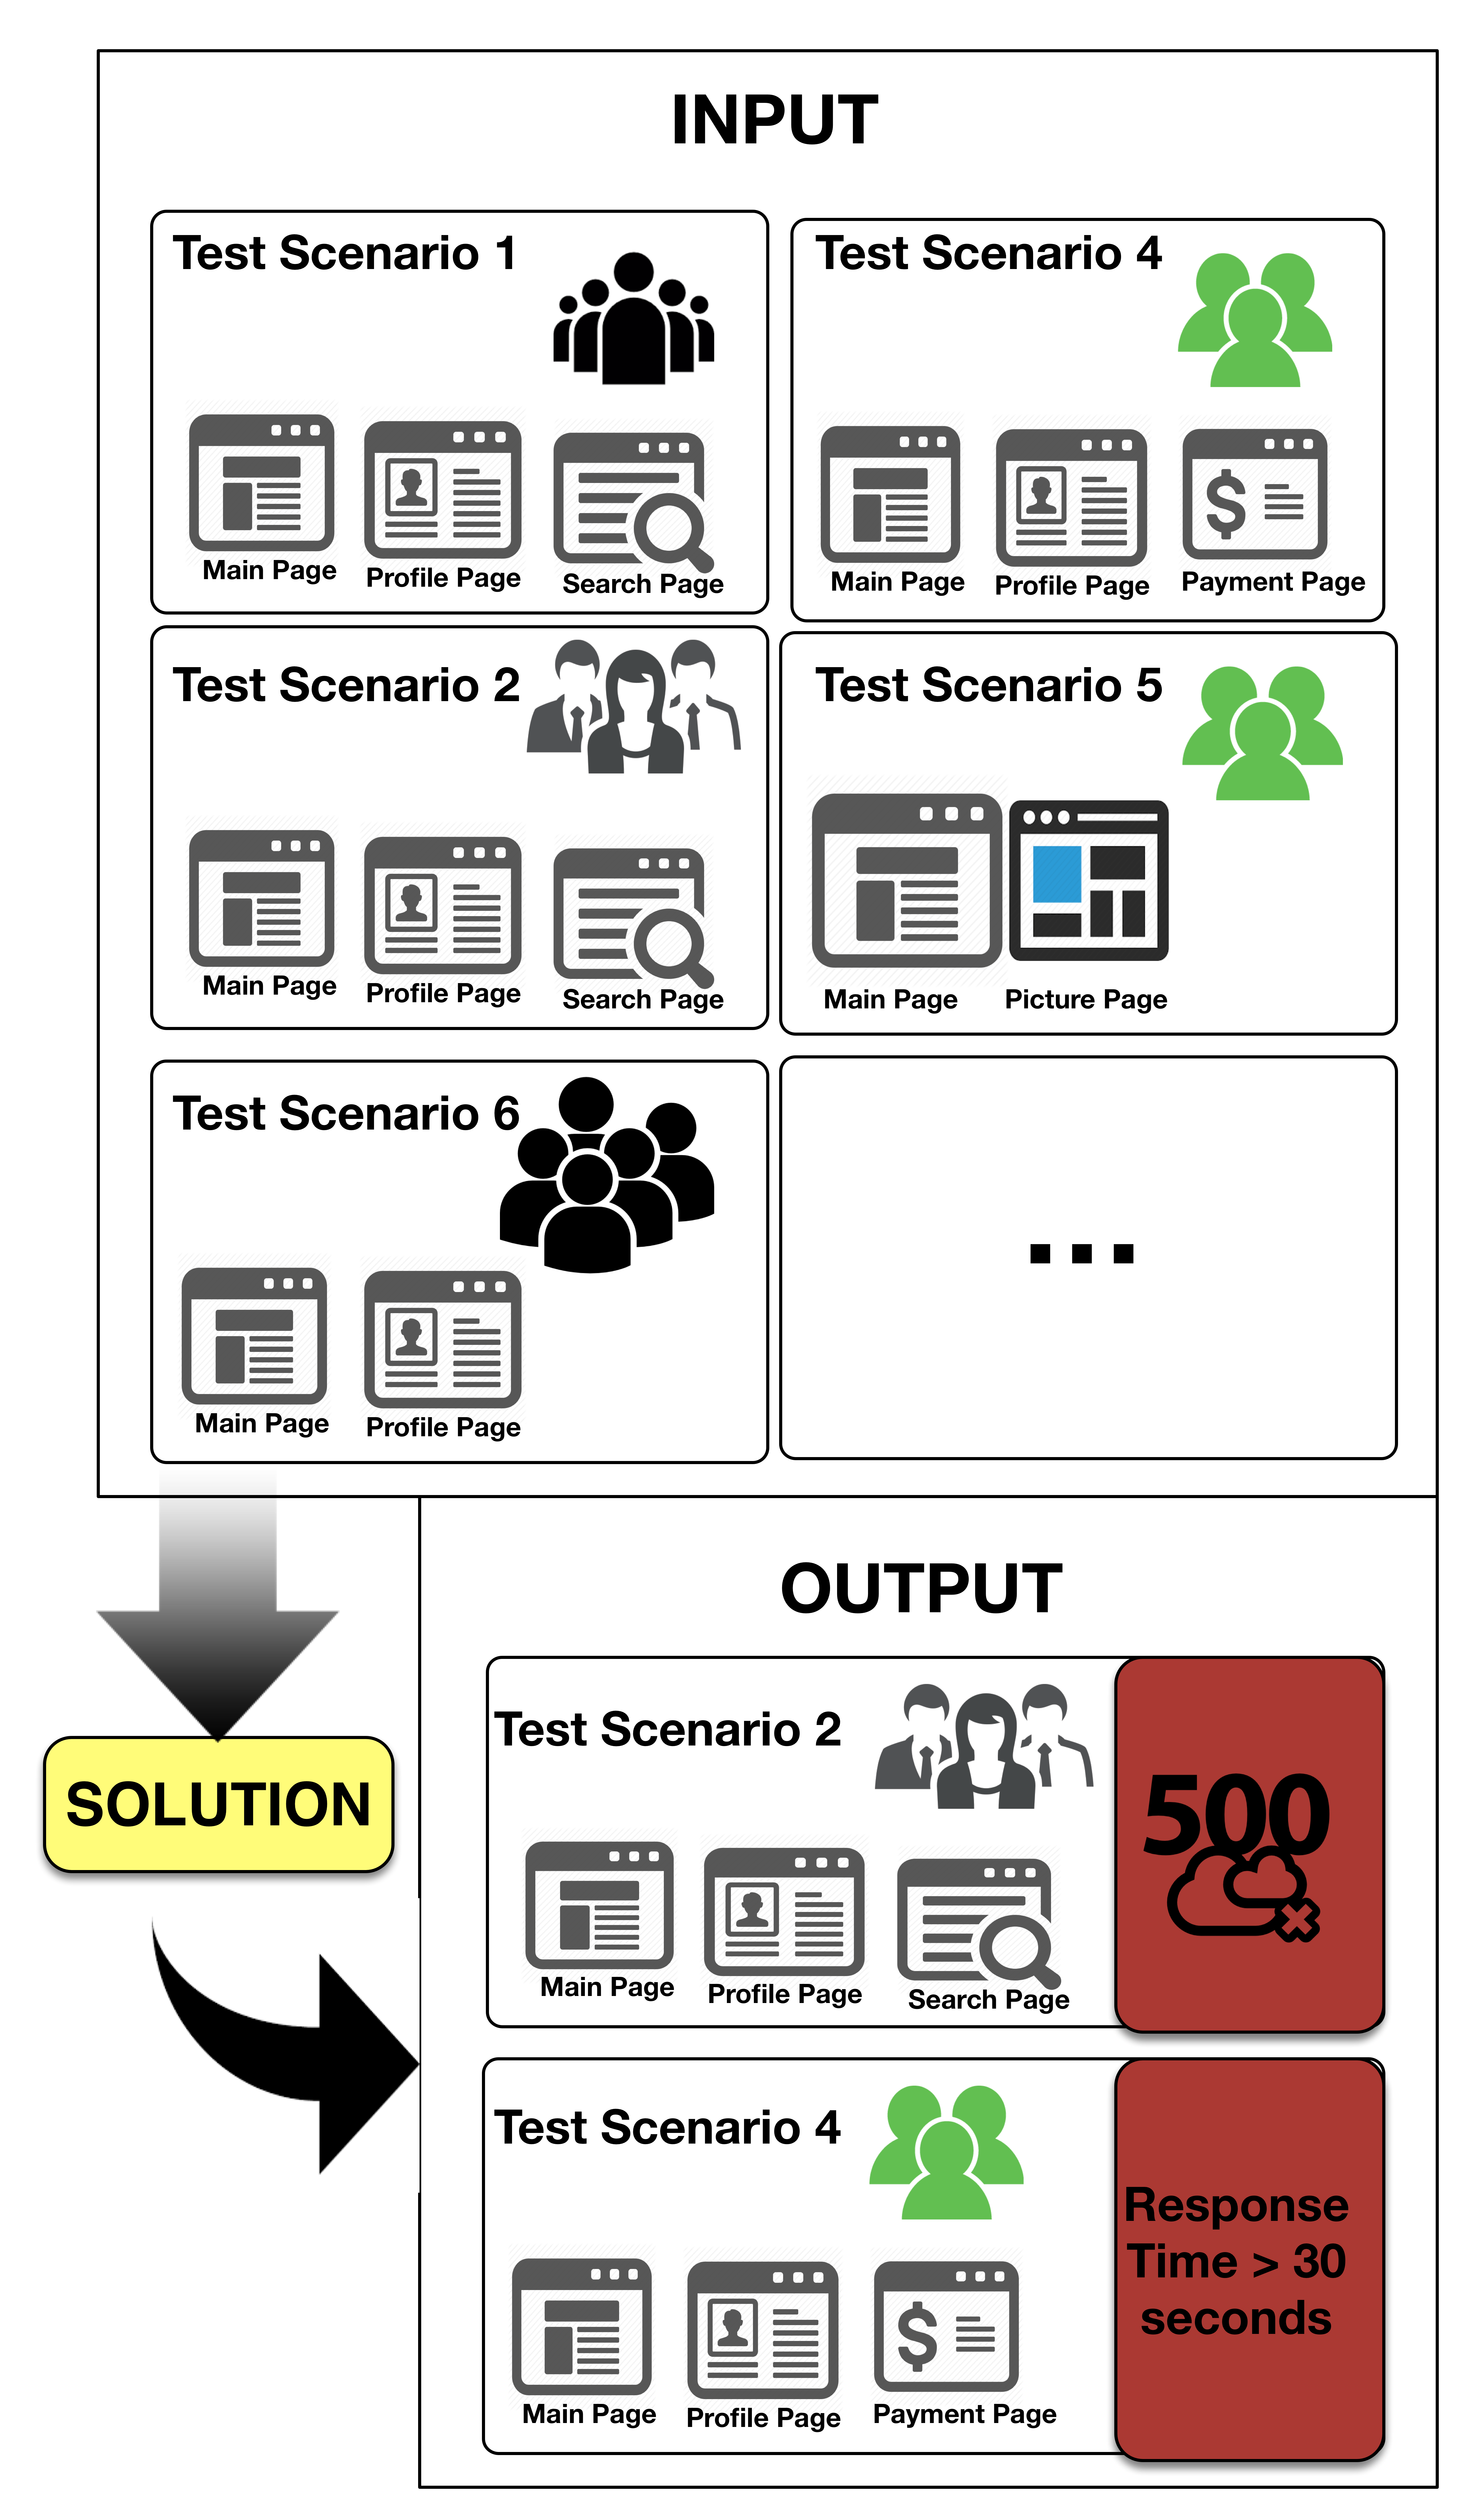
\includegraphics[width=0.35\textwidth]{./images/solution.png}
\label{fig:solution}
\end{figure}



% * <naubergois@gmail.com> 2015-09-17T00:49:26.764Z:
%
%  Rever paragrafo abaixo
%
%
The paper proposes the use of a approach using  hybrid metaheuristc  with  Genetic Algorithms, Simulated Annealing and Tabu Search Algorithms  in load, performance and stress evolutionary tests.

A tool named IAdapter, a JMeter Plugin to perform Search Based load, Performance or Stress tests, was developed. Two experiments were conducted to validate the proposed approach. The first experiment has been applied in an emulated component and the second one has been applied in an installed Moodle application.

The remainder of the paper is organized as follows. Section 2 presents a brief introduction in load, performance and stress tests. Section 3 presents concepts about WorkLoad Model. Section 4 presents concepts about Hybrid Metaheuristcs. Section 5 presents the research proposed approach. Section 6 presents The IAdapter tool. Section 7 discusses the related work. The Section 8 shows the results of two experiment applied with IAdapter. Conclusions and further work are presented in Section 9.